
\section{Event Categorization}
\label{sec:categorization}
\subsection{Event Categories targeting production mechanisms}
%The selected events are classified into mutually exclusive categories designed to have best sensitivity for STXS Stage-1 measurement.
In order to probe different Higgs boson production mechanisms, the selected events are classified into mutually exclusive categories. Seven categories are defined in the same way as previous Run2 analyses~\cite{CMS-PAS-HIG-18-001}, except that in the VBF-1jet-tagged category, ${\cal D}_{\rm 1jet}$ requirement is shifted from 0.5 to 0.7 to improve the purity. The criteria is applied in this exact order as follows (i.e. an event is considered for the subsequent category only if it does not satisfy the requirements of the previous category):
\begin{itemize}
\item {\bf VBF-2jet-tagged category} requires exactly 4 leptons. In addition there must be either 2 or 3 jets of which at most 1 is b-tagged, or at least 4 jets and no b-tagged jets. Finally, ${\cal D}_{\rm 2jet}>0.5$ is required.
\item {\bf VH-hadronic-tagged category} requires exactly 4 leptons. In addition there must be 2 or 3 jets, or at least 4 jets and no b-tagged jets. Finally, ${\cal D}_{\rm VH} \equiv {\rm max}({\cal D}_{\rm ZH},{\cal D}_{\rm WH})>0.5$ is required.
\item {\bf VH-leptonic-tagged category} requires no more than 3 jets and no b-tagged jets in the event,
and exactly 1 additional lepton or 1 additional pair of opposite sign same flavor leptons. This category also includes events
with no jets and at least 1 additional lepton.
\item {\bf t$\mathbf{\bar{t}}$H-hadronic-tagged category} requires at least 4 jets of which at least 1 is b-tagged and no additional leptons.
\item {\bf t$\mathbf{\bar{t}}$H-leptonic-tagged category} requires at least 1 additional lepton in the event.
\item {\bf VBF-1jet-tagged category} requires exactly 4 leptons, exactly 1 jet and ${\cal D}_{\rm 1jet}>0.5$.
\item {\bf Untagged category} consists of the remaining events.
\end{itemize}
Figure~\ref{fig:categ-purity} shows the event yields in the seven categories calculated using 2018 MC and scaled to full Run II luminosity.
%=======
\begin{figure}[!htb]
\vspace*{0.3cm}
\begin{center}
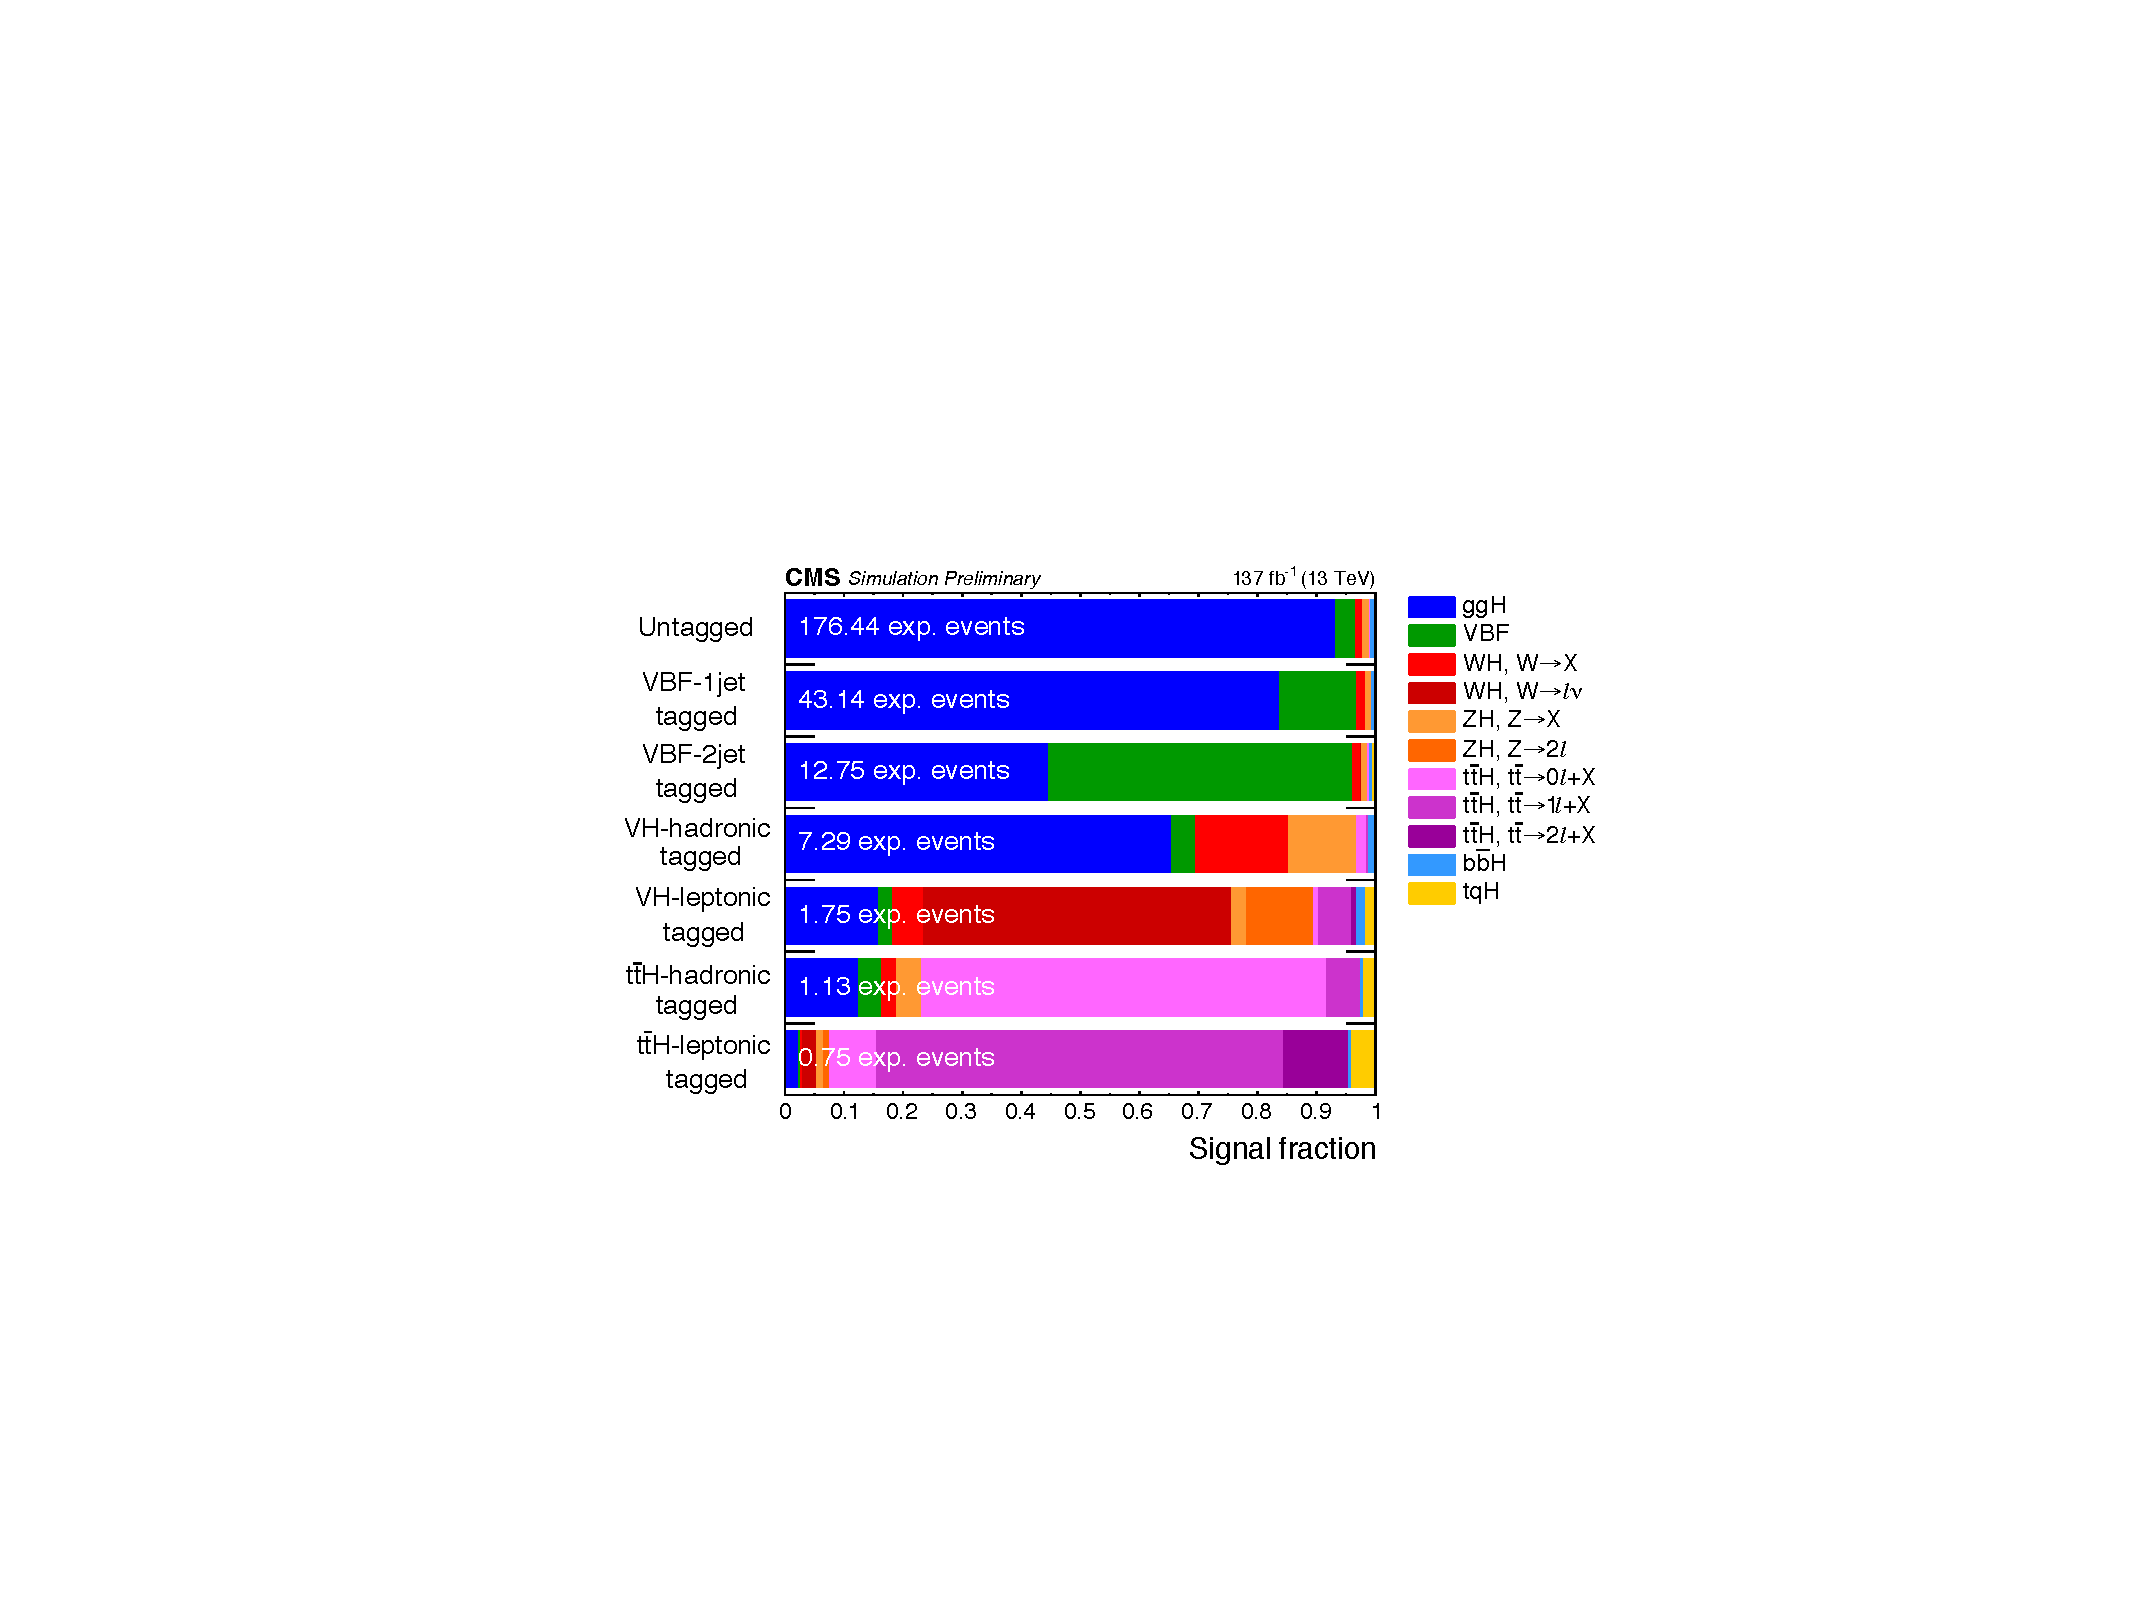
\includegraphics[width=0.8\textwidth]{Figures/stxs/Purity.pdf}
\caption{Signal relative purity of the seven event categories in terms of the seven main production mechanisms of the Higgs boson in a $118<\mllll<130\GeV$ mass window. The $\WH$, $\ZH$ and $\ttH$ processes are split according to the decay of associated objects, whereby X denotes anything other than an electron or muon.
\label{fig:categ-purity}}
\end{center}
\end{figure}
%=======
~
\subsection{Finer Event Categories targeting simplified template cross sections}
\label{subsec:stxs_cat}
Simplified template cross sections (STXS)~\cite{STXSstage11} were developed to provide finely-grained measurements than signal strength and multiplicative coupling modifiers. The primary goals of the STXS framework are to maximize the sensitivity of the measurements while at the same time to minimize their theory dependence. The measured exclusive regions of phase space, called bins for simplicity, are specific to the different production modes. To account for the evolving experimental sensitivity, the STXS bins are defined in stages (corresponding to increasingly fine granularity). The stage 0 bins correspond to the Higgs boson production mechanisms. The previous Run2 analysis has reported the measured stage 0 results~\cite{CMS-PAS-HIG-18-001}. With full Run2 data, this analysis targets the finer stage 1.1 bins. The bin definitions are shown in Figure~\ref{fig:stage1_ggH},~\ref{fig:stage1_VBF} and ~\ref{fig:stage1_VH} for ggF, VBF and VH productions, respectively. 
%=======
\begin{figure}[!htb]
  \vspace*{0.3cm}
  \begin{center}
    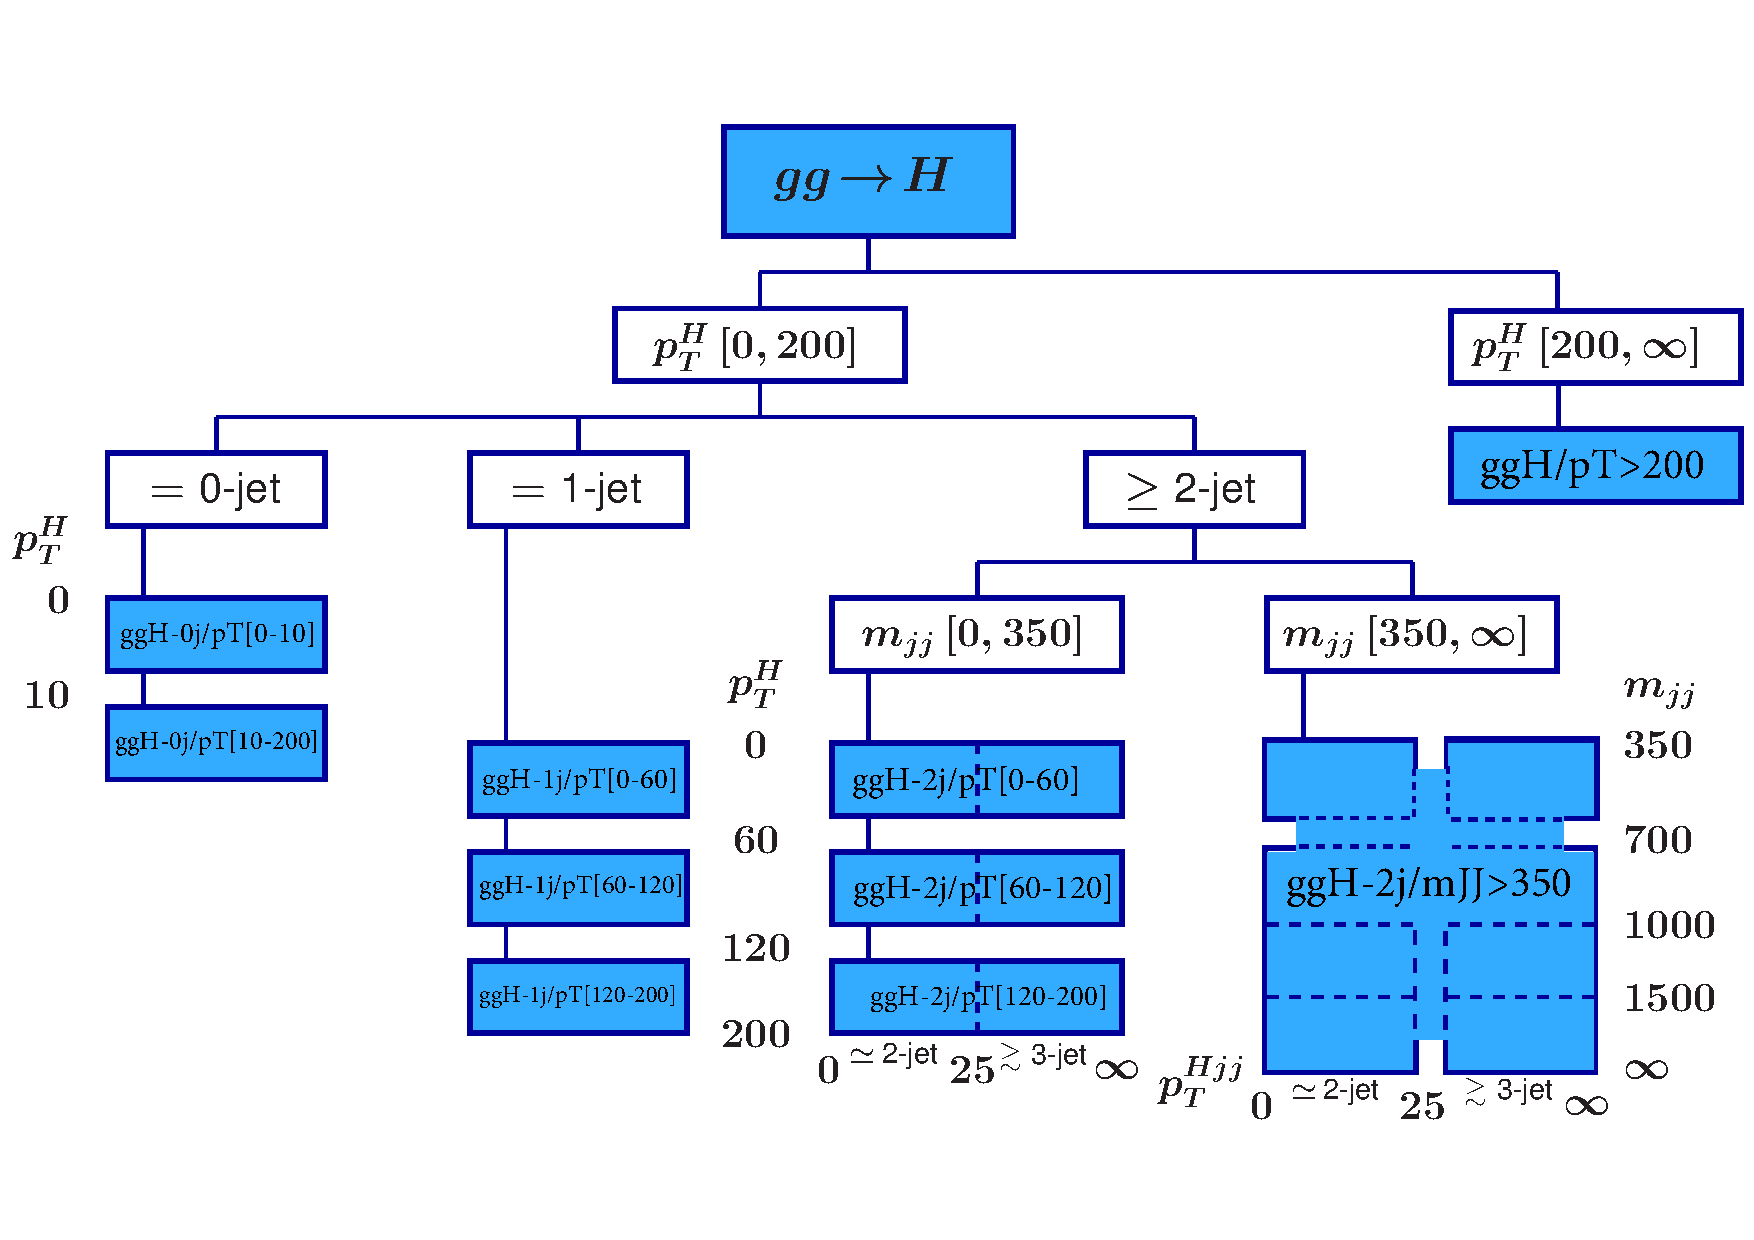
\includegraphics[width=0.8\textwidth]{Figures/stxs/simplifiedXS_ggF_11.pdf}
    \caption{STXS stage 1.1 definition for ggF production mechanism.} 
    \label{fig:stage1_ggH}}
      \end{center}
\end{figure}
%=======
%=======
\begin{figure}[!htb]
  \vspace*{0.3cm}
  \begin{center}
    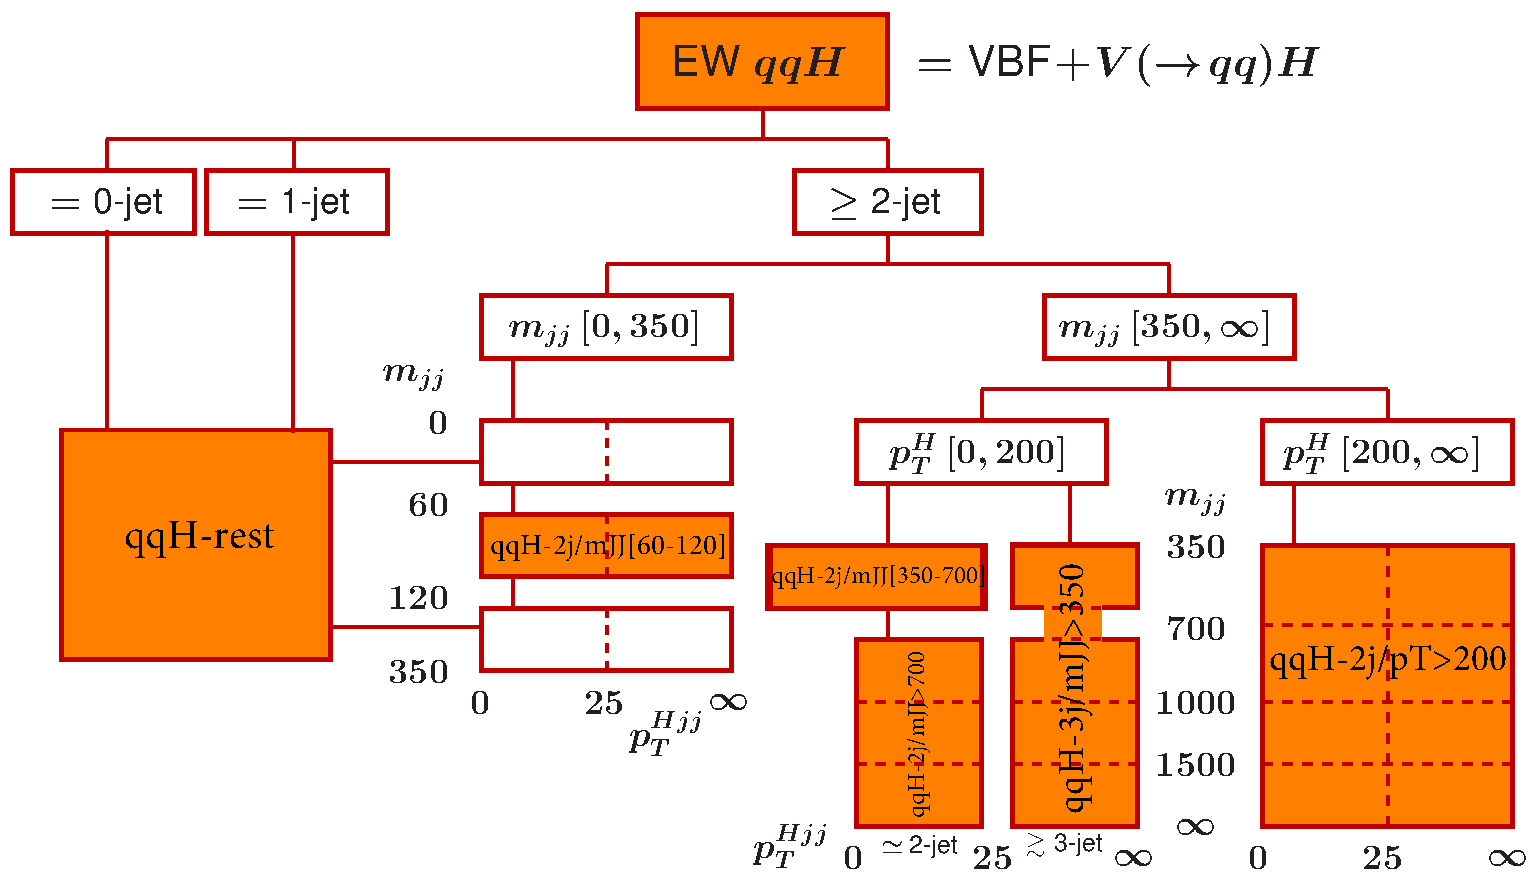
\includegraphics[width=0.8\textwidth]{Figures/stxs/simplifiedXS_VBF_11.pdf}
    \caption{STXS stage 1.1 definition for VBF production mechanism.} 
    \label{fig:stage1_VBF}}
      \end{center}
\end{figure}
%=======
%=======
\begin{figure}[!htb]
  \vspace*{0.3cm}
  \begin{center}
    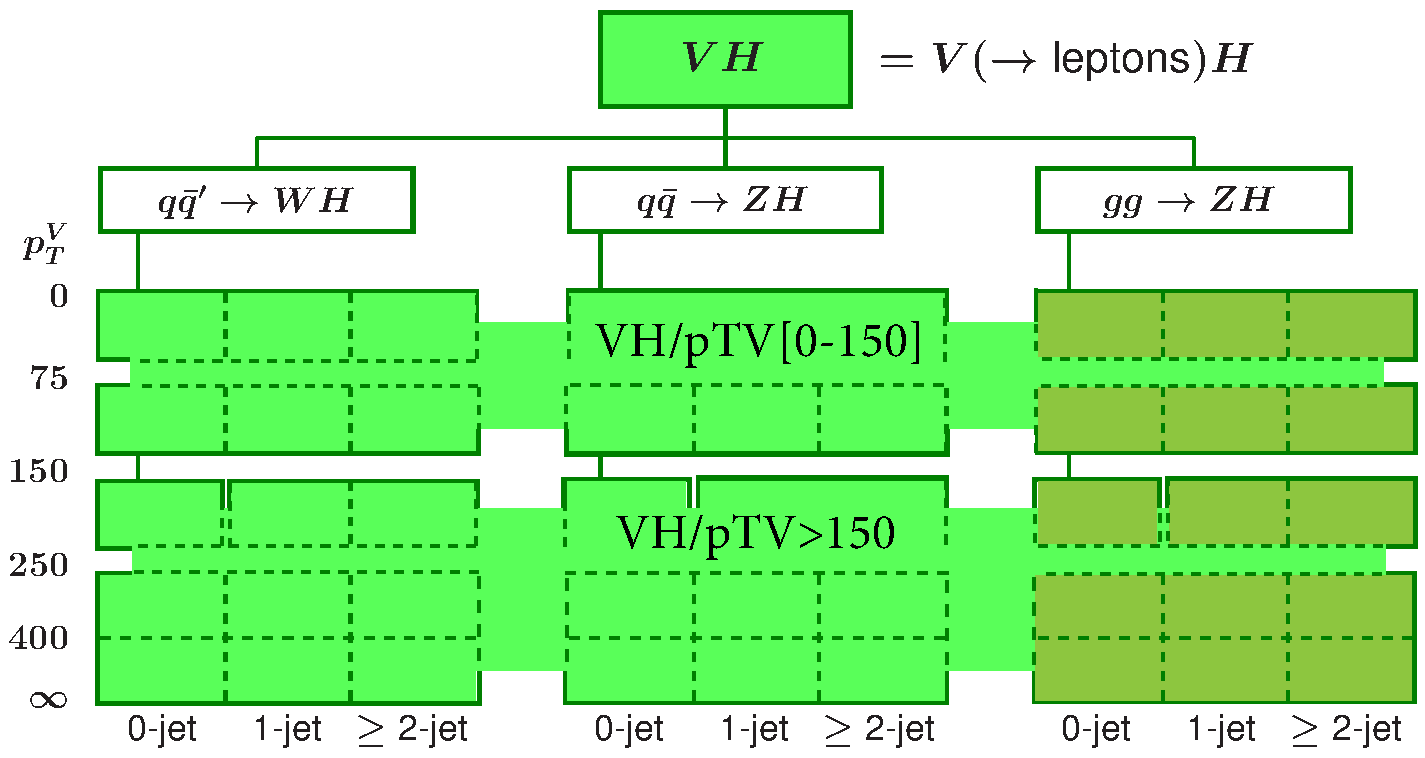
\includegraphics[width=0.8\textwidth]{Figures/stxs/simplifiedXS_VH_11.pdf}
    \caption{STXS stage 1.1 definition for VH production mechanism.} 
    \label{fig:stage1_VH}}
      \end{center}
\end{figure}
%=======
Figure~\ref{fig:yield_stage11_all} shows the expected signal event yields at 136.2 \fbinv of all stage 1.1 bins reconstructed. Some of the stage 1.1 bins expect less than 1 event, thus the analysis is not sensitive to them. These bins are merged and the measurement is provided for the merged bins. More specifically, ggF 2jets and 3 jets bins above $m_{jj} > 350$ \GeV are merged to one; two bins of VBF 3 jets ($350 < m_{jj} < 700$ GeV and $m_{jj} > 700$\GeV) are merged to one; WH and ZH bins are merged as one VH bin, and only splitted to $p_{T}^{V}<150$ \GeV and $p_{T}^{V}>150$ \GeV bins. 
%=======
\begin{figure}[!htb]
        \vspace*{0.3cm}
        \begin{center}
                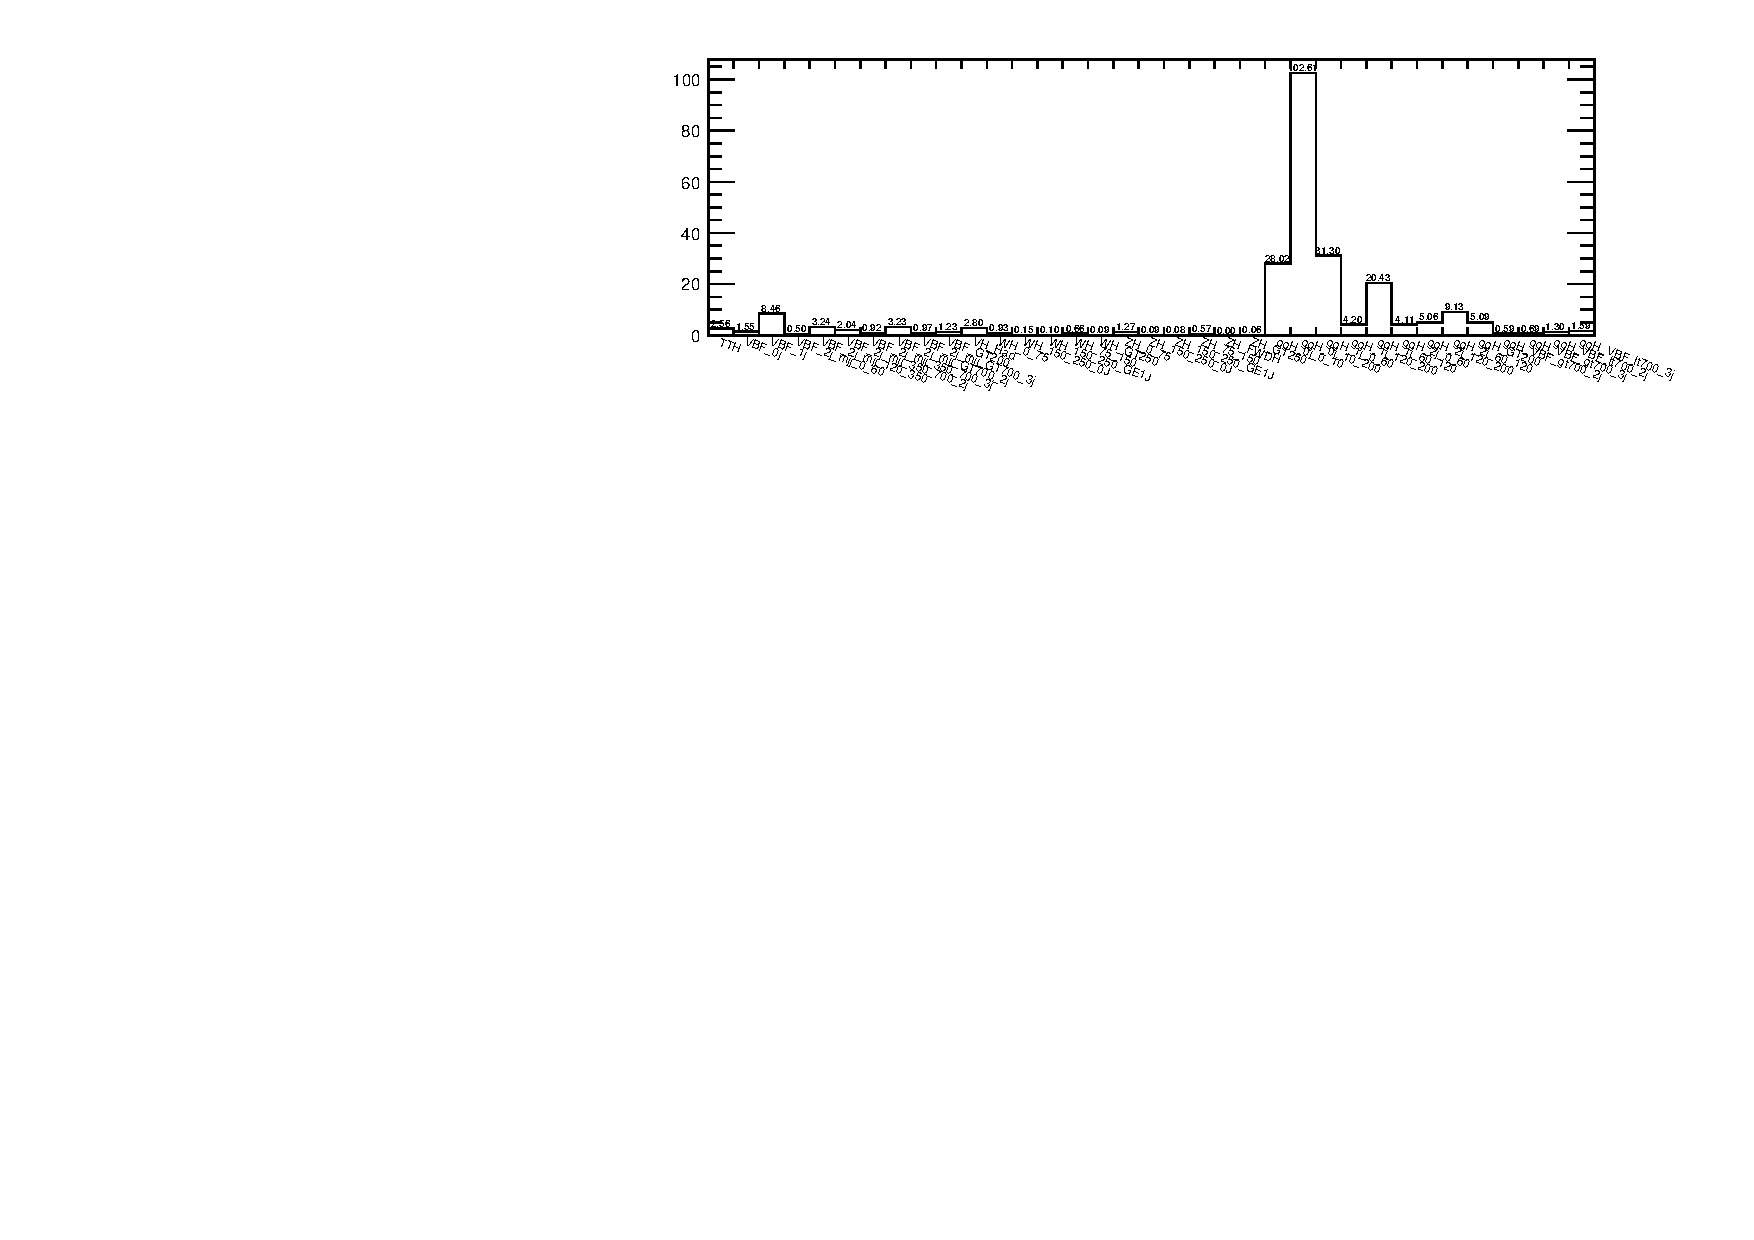
\includegraphics[width=0.95\textwidth]{Figures/stxs/moriond_stage1p1_all_all.pdf}
                \caption{Expected signal event yields at 136.2 \fbinv of all stage 1.1 bins reconstructed.}
                \label{fig:yield_stage11_all}}
        \end{center}
\end{figure}
%=======
To maximize the sensitivity to the stage 1.1 bins, the above 7 reconstructed categories are further splitted into 22 categories.  
\begin{itemize}
\item {\bf Untagged category}
\begin{enumerate}
\item{ggH-PTH-200}: if \pt of the Higgs is $> 200$ \GeV 
\item{ggH-0J-PTH-0-10}: if 0 jet reconstructed and the Higgs \pt is between [0,10] \GeV  
\item{ggH-0J-PTH-10-200}: if 0 jet reconstructed and the Higgs \pt is between [10,200] \GeV  
\item{ggH-1J-PTH-0-60}: if 1 jet reconstructed and the Higgs \pt is between [0,60] \GeV  
\item{ggH-1J-PTH-60-120}: if 1 jet reconstructed and the Higgs \pt is between [60,120] \GeV  
\item{ggH-1J-PTH-120-200}: if 1 jet reconstructed and the Higgs \pt is between [120,200] \GeV  
\item{ggH-VBF}: if 2 jets reconstructed and $m_{jj} >$ 350\GeV 
\item{ggH-2J-PTH-0-60}: if 2 jets reconstructed and the Higgs \pt is between [0,60] \GeV and not ggH-VBF 
\item{ggH-2J-PTH-60-120}'' if 2 jets reconstructed and the Higgs \pt is between [60,120] \GeV and not ggH-VBF
\item{ggH-2J-PTH-120-200}: if 2 jets reconstructed and the Higgs \pt is between [120,200] \GeV and not ggH-VBF
\end{enumerate}
\item {\bf VBF-1jet-tagged category}
\item {\bf VBF-2jet-tagged category}
\begin{enumerate}
\item{VBF-GT200-2J}: if the Higgs \pt is $> 200$ \GeV and $m_{jj} >$ 350\GeV
\item{VBF-2j-mjj-350-700}: if the Higgs \pt is $< 200$ \GeV, $p_T^{Hjj}<25$\GeV, $m_{jj}$ is between [350,700]\GeV 
\item{VBF-2j-mjj-GT700j}: if the Higgs \pt is $< 200$ \GeV, $p_T^{Hjj}<25$\GeV, $m_{jj}$ is $>700$\GeV 
\item{VBF-3j}: if the Higgs \pt is $< 200$ \GeV, $p_T^{Hjj}>25$\GeV, $m_{jj}>350$\GeV 
\item{VBF-2j}: if not above 
\end{enumerate}
\item {\bf VH-hadronic-tagged category}
\begin{enumerate}
\item{VH-Had} if $60<m_{jj}<120$\GeV 
\item{VBF-rest-VH}: not above 
\end{enumerate}
\item {\bf VH-leptonic-tagged category} 
\begin{enumerate}
\item{VH-lep-0-150}: if $p_T^{V} < 150$\GeV 
\item{VH-lep-GT150}: if $p_T^{V} > 150$\GeV 
\end{enumerate}
\item {\bf t$\mathbf{\bar{t}}$H-hadronic-tagged category} 
\item {\bf t$\mathbf{\bar{t}}$H-leptonic-tagged category}
\end{itemize}
Figure~\ref{fig:categ-purity-stage11} shows the signal relative purity of all STXS Stage 1.1 Bins in the 22 event sub-categories defined above.
%=======
\begin{figure}[!htb]
  \vspace*{0.3cm}
  \begin{center}
    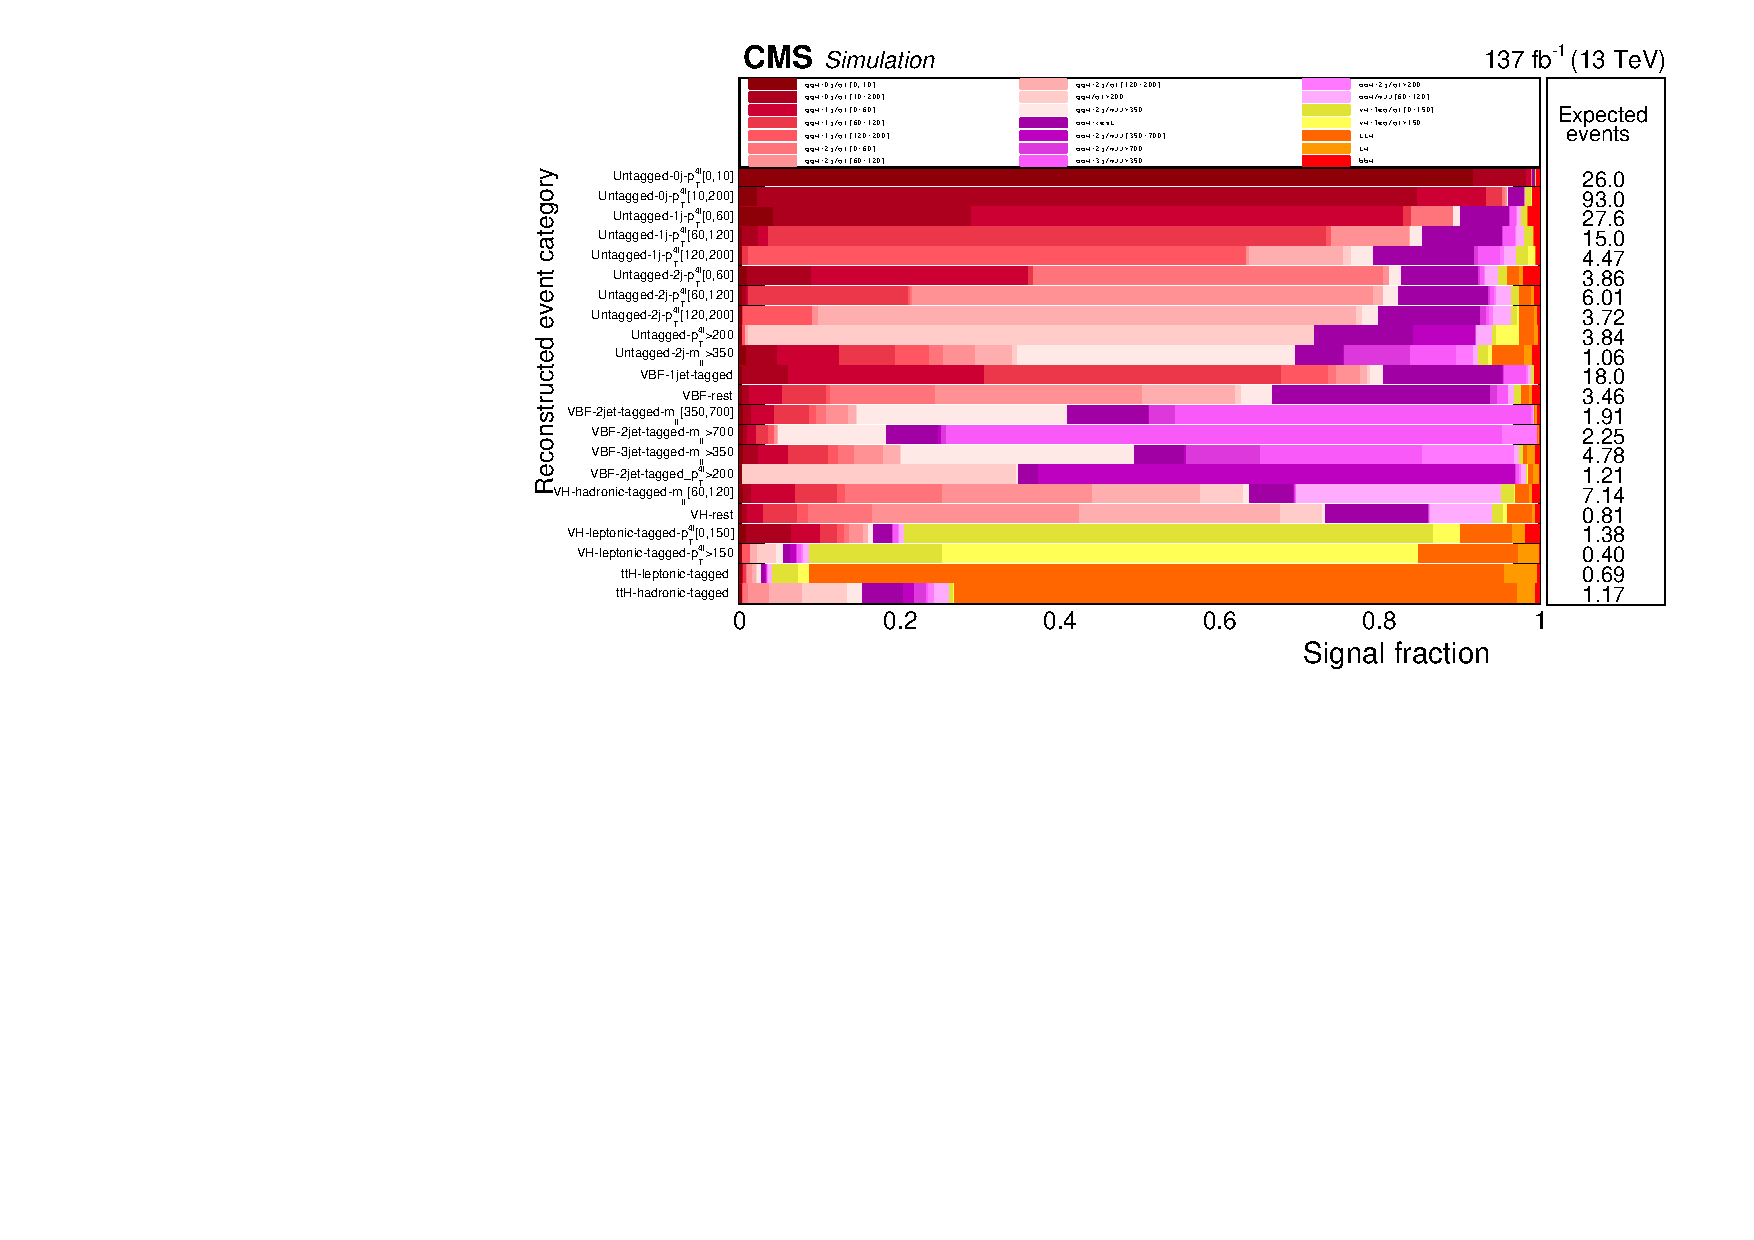
\includegraphics[width=0.95\textwidth]{Figures/stxs/STXS_Purity.pdf}
    \caption{Signal relative purity of the 22 event sub-categories in terms of the STXS Stage 1.1 Bins in a $118<\mllll<130\GeV$ mass window.
      \label{fig:categ-purity-stage11}}
    \end{center}
\end{figure}
%=======
%Figure~\ref{fig:stage1_cov} shows the expected yields of the reduced version of stage 1.1 bins in the 22 reconstructed categories.
%=======
%\begin{figure}[!htb]
%        \vspace*{0.3cm}
%        \begin{center}
%                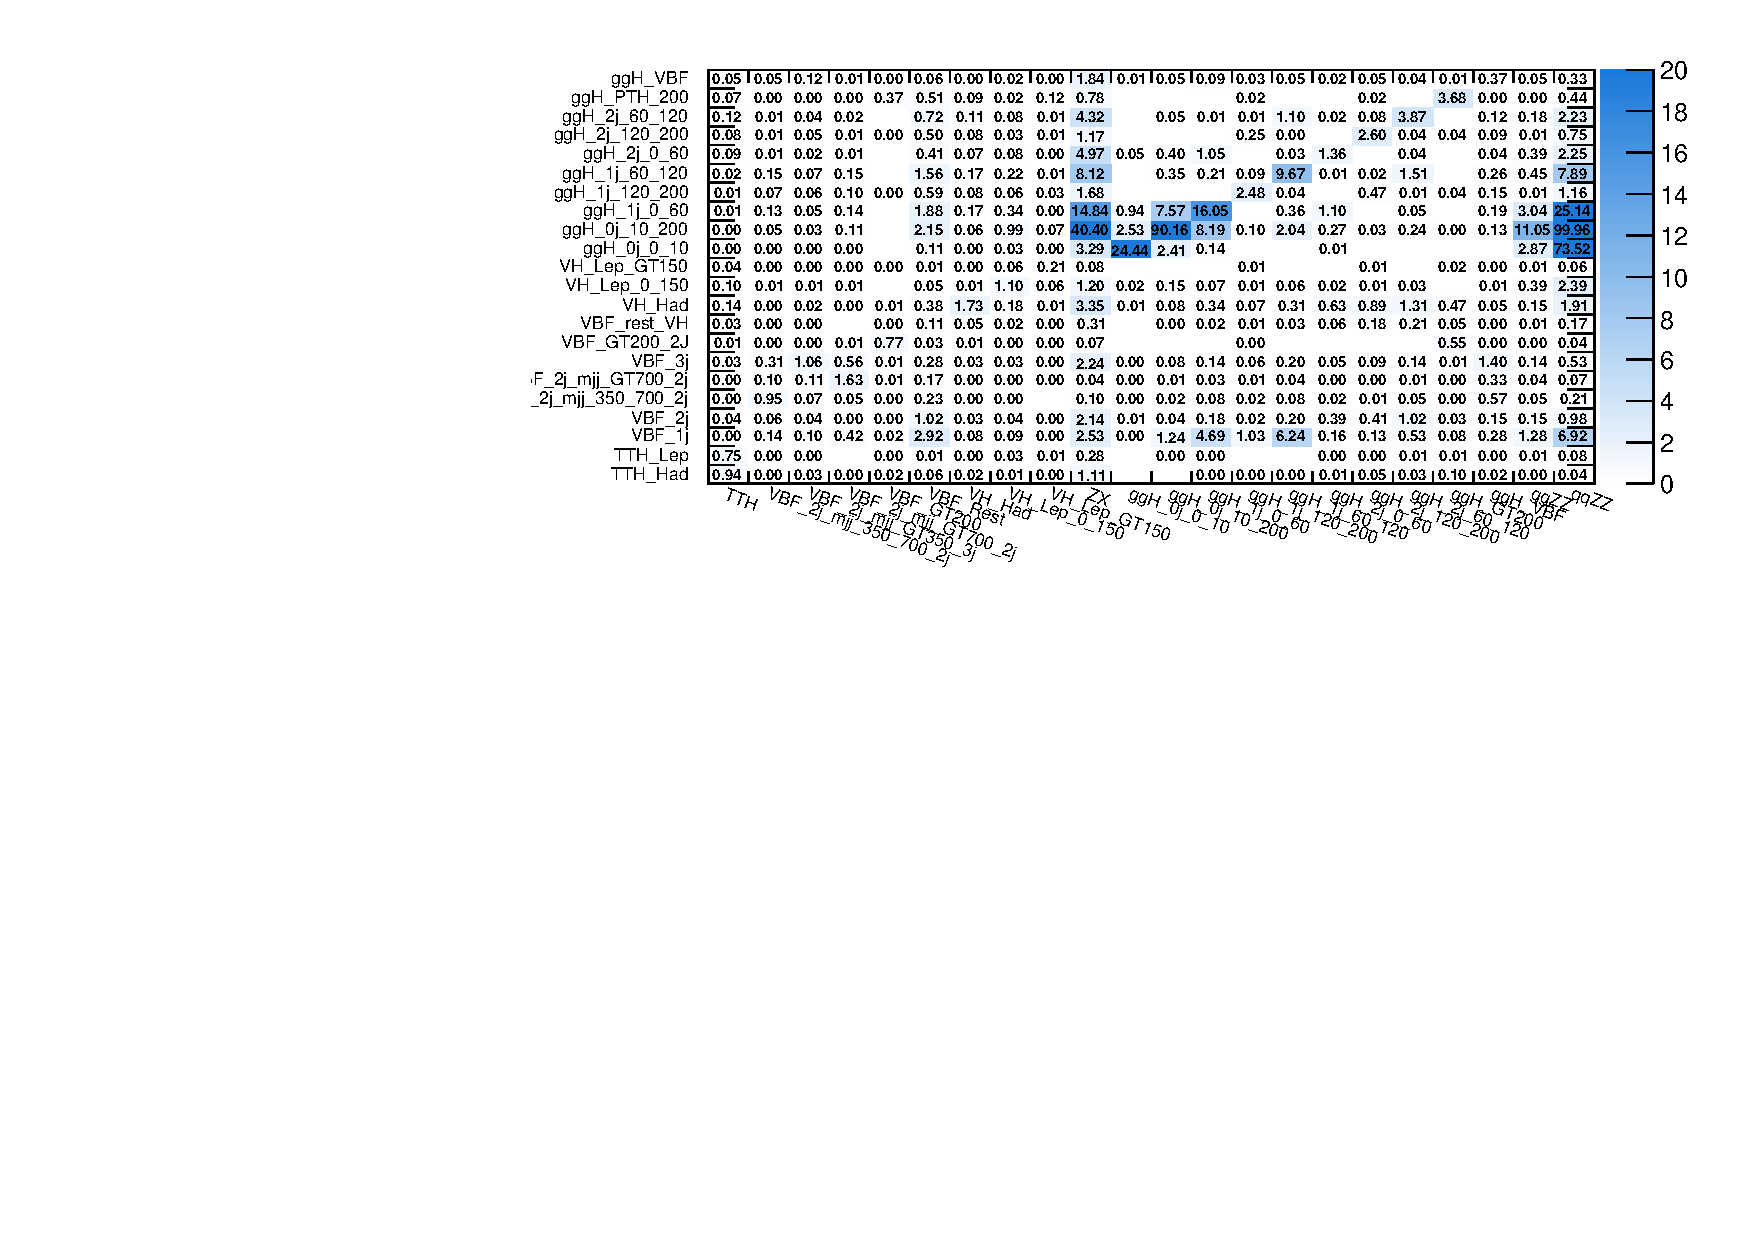
\includegraphics[width=0.95\textwidth]{Figures/stxs/moriond_stage1p1_all.pdf}
%                \caption{Expected yields of signal and background events in the reduced version of STXS stage-1.1 approach, combining 2016, 2017 and 2018 data.
%The x-axis indicates 20 signal and 2 background processes defined at MC-truth level. The y-axis indicates 22 reconstructed categories 
%optimized for various types of signal production modes. While the reconstructed categories and signal processes are designed to be close
%in definition, there is no one-to-one correspondence due to experimental topology selection (e.g. one ttH process is targeted by both hadronic
%and leptonic ttH categories, as indicated in the bottom-left corner). }
 %               \label{fig:stage1_cov}}
 %       \end{center}
%\end{figure}
%=======
